\subsection{Expressive Range Analysis}

\begin{table*}[ht]
% \centering
\caption{General consensus on EDD's features} \label{p1tab:consensus}
\resizebox{0.8\textwidth}{!}{
\begin{tabularx}{\textwidth}{|p{0.2\textwidth}|p{0.99\textwidth}|}
\cline{1-2}

Description & Participants’ Consensus \\\cline{1-2}
World Grid  of the dungeon                   & Its purpose of establishing an illusion of a fully realized dungeon is somewhat achieved. However, limitations exist with how it defines feasibility, a dungeon’s starting point, and the entrances, which disrupts the designers’ decisions.                                                                                                                                                                                   \\\cline{1-2}
World View                                  & The world view’s usefulness for the most part could not be established, other than for the purpose of going to the suggestions view (which was already seldom during the user study) and having a closer look at the entire dungeon without any distractions. Some participants preferred features to be already in the room view’s minimap, and some wanted to see more specific functionalities within the world view itself. \\\cline{1-2}

Enabling and  \newline disabling rooms                & As the user study restricted participants to create 3x3 dungeons, this feature for the most part has been neglected. This is also in part because of its accessibility only being in the world view, which proved to be an inefficient view in general. However, its use for bigger dungeon sizes later on was appreciated, especially for more intricate design purposes.                                                      \\\cline{1-2}
Suggestions View                            & Similarly to enabling and disabling rooms, it was quite difficult to encourage the use of this functionality due to the world view’s inefficient usability. However, this could also be due to the dungeon’s small size, as some participants expressed high interest in using more suggestions with larger dungeon sizes.                                                                                                      \\\cline{1-2}
Minimap  \newline  navigation                      & The minimap proved to be a strong tool not only for navigation purposes, but also for supporting design decisions and choices. The directional buttons were rarely used, but their room previews were helpful in emphasizing the current room’s connection to adjacent rooms without looking at the minimap. On the other hand, this lowered the usability of the world view.                                                   \\\cline{1-2}
Parameters                                       & The parameters were, in general, lacking. They served to be important in decision-making when choosing a suggested map in room view, but there were still doubts on their accuracy and sufficiency when providing information about the generated suggestions.                                                                                                                                                                       \\\cline{1-2}
Generated maps for  \newline  suggestions in room view & Suggestions in the room view proved to be very helpful in supporting the whole design process as they primarily acted as inspirations for the users. The most prominent comment among the users is the preference of having more control on how suggestions should be generated depending on different types of parameters.                                                                                                     \\\cline{1-2}
Design \newline  patterns& The patterns’ visualization was, in general, lacking and not self-explanatory. Some participants have expressed interest in using patterns as a parameter in the generation of suggestions.                                                                                                                                                                                                                                     \\\cline{1-2}
Dark theme                                  & EDD’s dark theme for the user interface received a positive response as it makes working with the program easier.
	\\ \cline{1-2}
\end{tabularx}
}
\end{table*}

% \begin{table}
% \begin{center}
% {\caption{Best performing setups based on their internal validation and visualization of clustered data points.}\label{table:setups}}
% \resizebox{\textwidth}{!}{
% \begin{tabular}{ccccccc}
% \hline
% \rule{0pt}{12pt}
% Algorithm&Data&K&$\Diamond$&$\Box$&$\bigtriangleup$ 
% \\ 
% \hline
% \\[-6pt]
% K-Means & Tiles-PCA & 9 & 0.43 & 0.73 & 9438.233 \\ 
% K-Means & Tiles-PCA & 12 & 0.41 & 0.77 & 9436.928 \\
% K-Means & Dimensions-PCA & 12 & 0.43 & 0.73 & 7738.343 \\
% Agglomerative single & Combined-PCA & 6 & 0.51 & 0.43  & 38.833 \\ 
% Agglomerative avg. & Dimensions-PCA & 6 & 0.44 & 0.67 & 3463.567 \\ 
% \hline
% \\[-6pt]
% \multicolumn{6}{l}{$\Diamond$ Silhouette Score\ \
% $\Box$ Davies Bouldin Index\ \
% $\bigtriangleup$ Calinski-Harabasz Index}
% \end{tabular}
% }\end{center}
% \end{table}

% \begin{table}[]
% \centering
% \caption{}
% \label{tab:my-table}
% % \resizebox{0.25\textwidth}{!}{%
% \begin{tabular}{|l|lll|}
% \hline
% Dimensions & \multicolumn{1}{c|}{$\Diamond$} & \multicolumn{1}{c|}{$\bigtriangleup$} & \multicolumn{1}{c|}{$\bigcirc$} \\ \hline
% IS-Sym         & 0.91 & 31.84\% & 42.7\%  \\
% Len-IS         & 0.9  & 32.28\% & 39.7\%  \\
% Len-Lin        & 0.9  & 34.7\%  & 47.6\%  \\
% Len-Sim        & 0.88 & 33.95\% & 41\%    \\
% Len-Sym        & 0.91 & 38.27\% & 56.5\%  \\
% Lin-IS         & 0.9  & 31.63\% & 38\%    \\
% Lin-Sim        & 0.88 & 32.6\%  & 40.8\%  \\
% Lin-Sym        & 0.91 & 32.51\% & 48.6\%  \\
% NMP-IS         & 0.89 & 33.58\% & 50.8\%  \\
% NMP-Len        & 0.89 & 38.32\% & 67.2\%  \\
% NMP-Lin        & 0.89 & 35.03\% & 56.6\%  \\
% NMP-NSP        & 0.88 & 36.32\% & 63.9\%  \\
% NMP-Sim        & 0.87 & 32.32\% & 36.9\%  \\
% NMP-Sym        & 0.89 & 33.33\% & 51.6\%  \\
% NSP-IS         & 0.89 & 32.94\% & 50.8\%  \\
% NSP-Len        & 0.89 & 38.32\% & 63\%    \\
% NSP-Lin        & 0.89 & 36.04\% & 44\%    \\
% NSP-Sim        & 0.86 & 34.31\% & 49.7\%  \\
% NSP-Sym        & 0.9  & 36.2\%  & 68.5\%  \\
% Sim-IS         & 0.87 & 30.75\% & 28.5\%  \\
% Sim-Sym        & 0.88 & 32.01\% & 43.2\%  \\ \hline
% Average        & 0.89 & 34.15\% & 49.03\% \\ \hline
% All Dimensions & 0.78 & 48.27\% & N/A      \\ \hline
% Traditional EA & 0.92 & 21.09\% & N/A      \\ \hline

% \multicolumn{4}{l}{$\Diamond$ Avg. Fitness \ \
% $\bigtriangleup$ Avg. covered space all dims} \\ 
% \multicolumn{4}{l}{$\bigcirc$ Covered search space in respective dimension pair}
% \end{tabular}%
% % }
% \end{table}

\begin{figure*}[h!]
\centerline{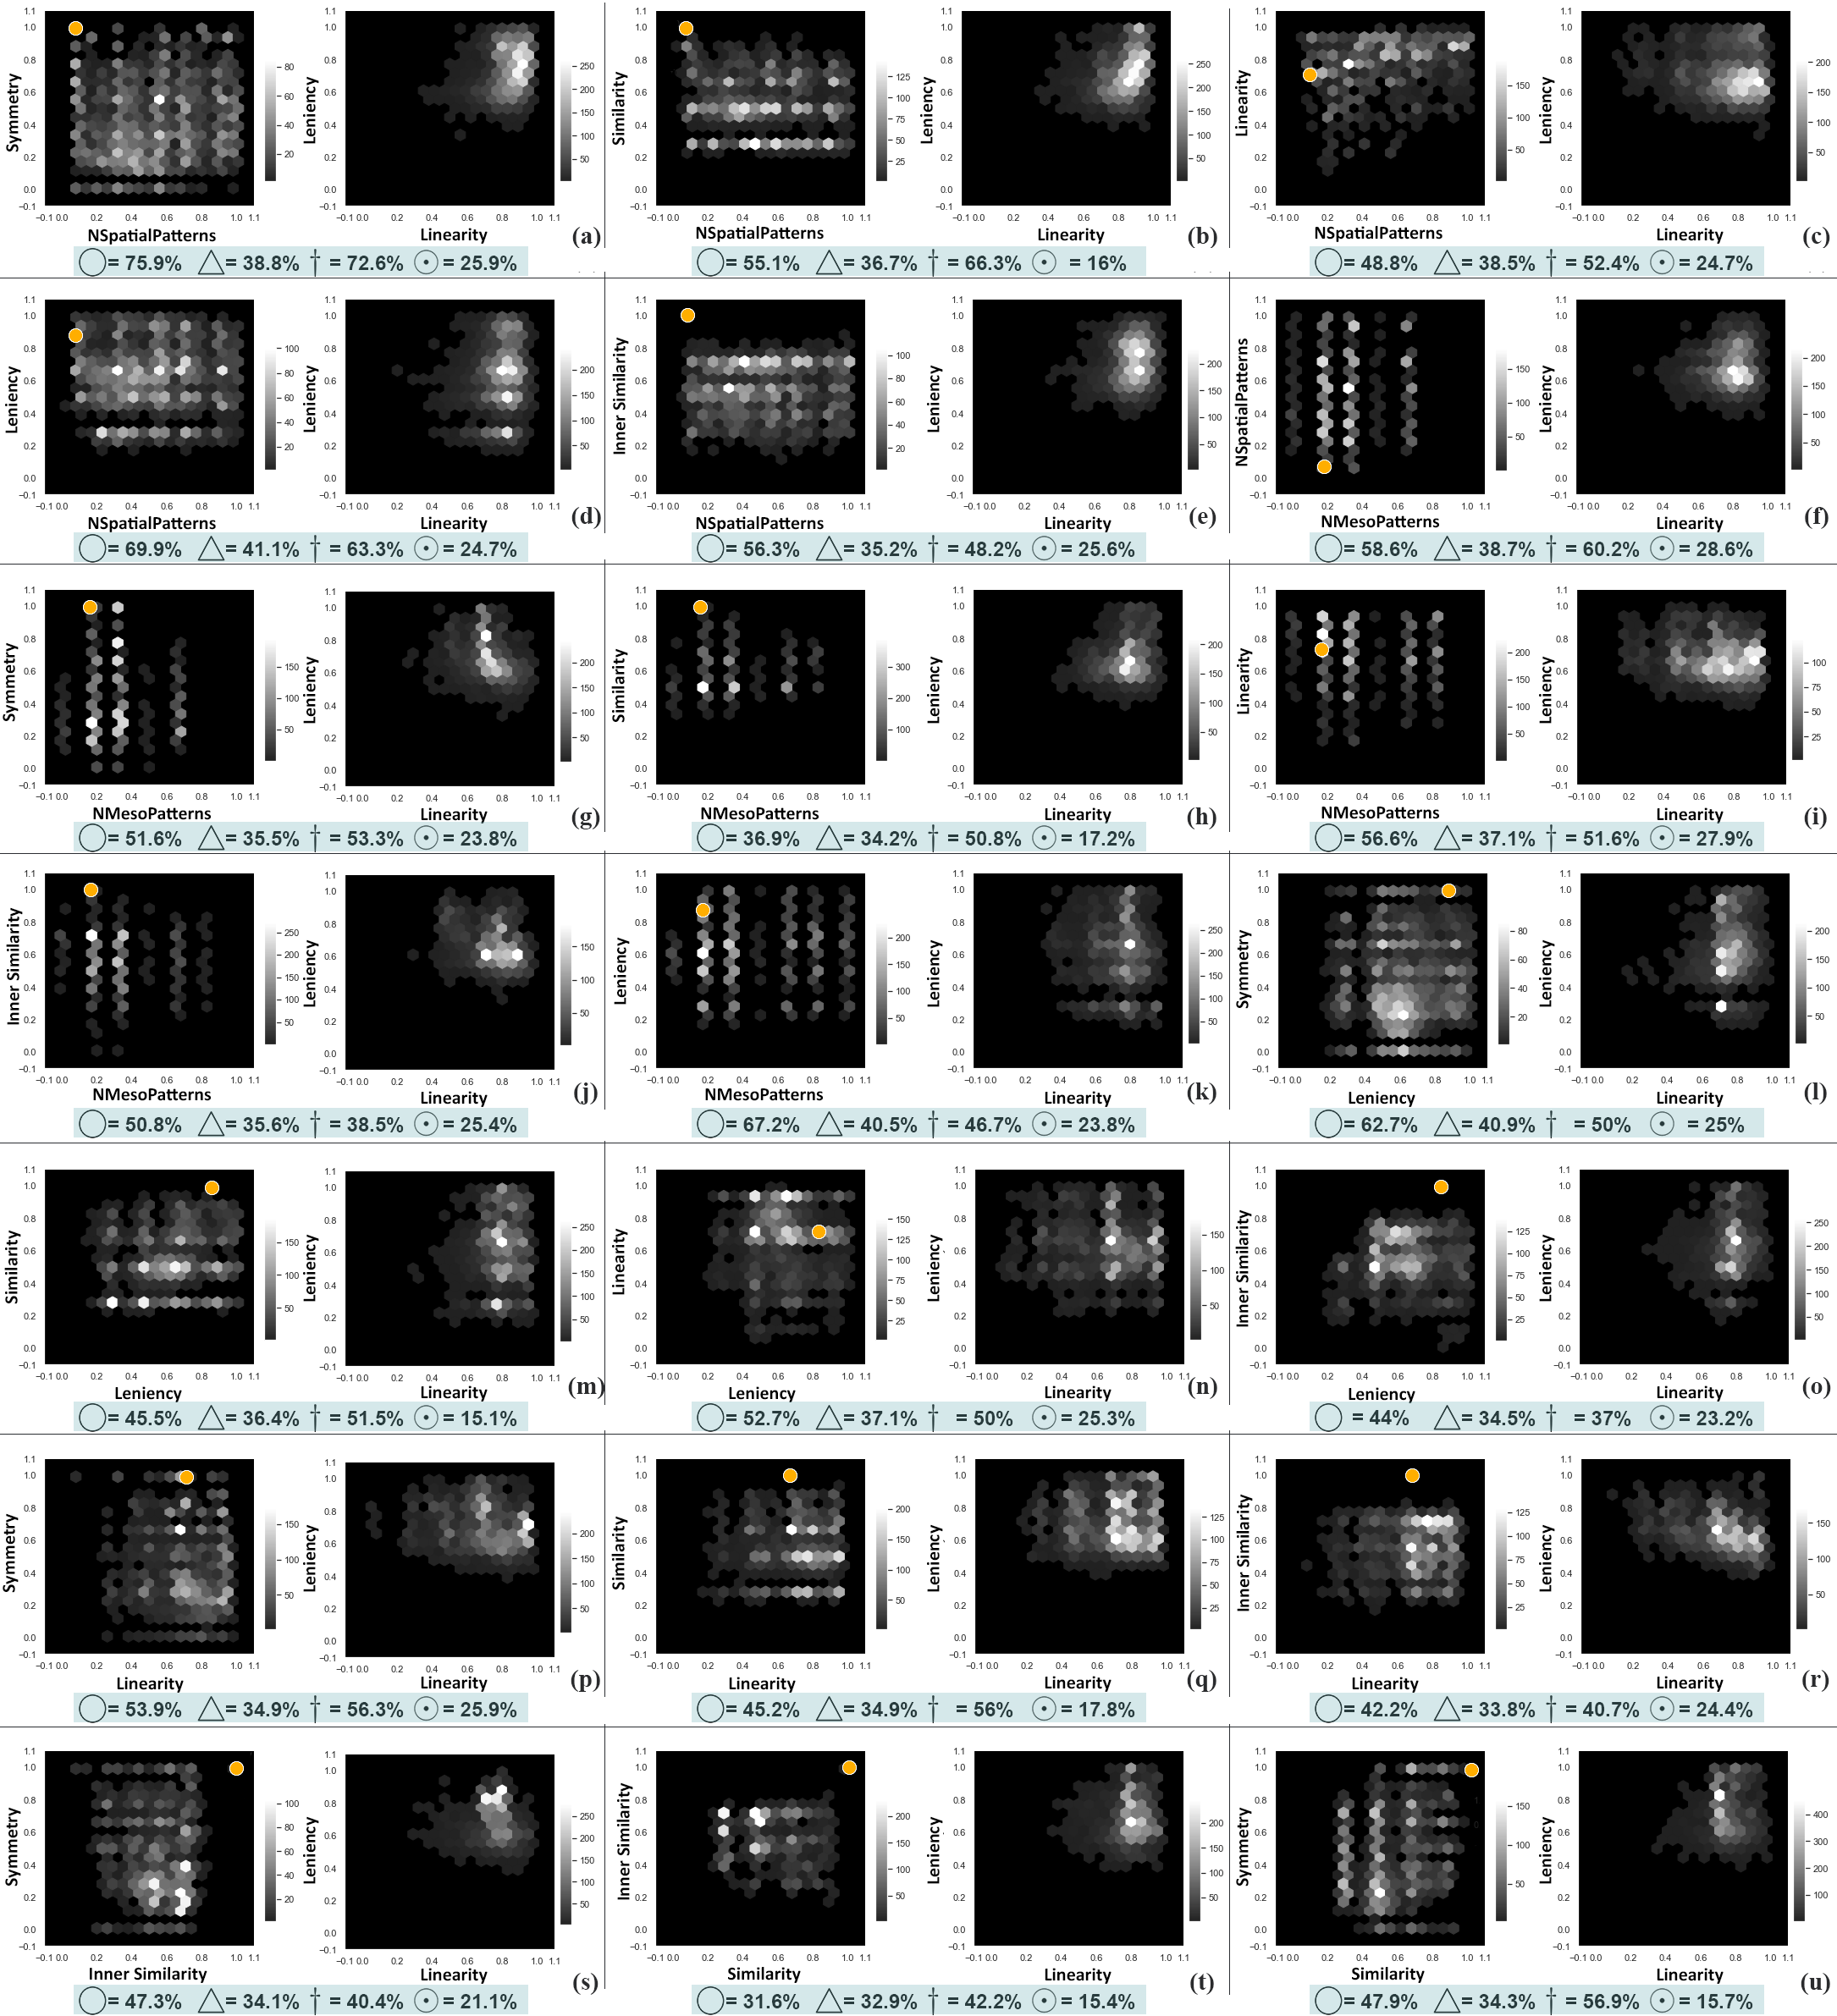
\includegraphics[width=15cm]{figures/figure4.png}}
\caption{Expressive range of the 21 possible combinations (from a to u) of dimensions picked in pairs. Each subfigure is composed of two plots: (left) an evaluation based on a given pair of dimensions; (right) the same pair of dimensions but evaluated in terms of Linearity and Leniency scores. Each hexagon relates to a dimensional score, whereas a lighter hue indicates a higher number of unique individuals generated under that particular score. All runs used~\Cref{figs:targetRoomsBas} as the target room, and its dimensional score is highlighted with an orange mark. Under each subfigure, we present data particular to the specific tested pair of dimensions. $\bigcirc$, $\dagger$, and $\odot$ represent the coverage percentage in the respective pair of dimensions when running IC MAP-Elites with the subfigure's pair of dimensions ($\bigcirc$), IC MAP-Elites with all dimensions in the search ($\dagger$), and when using objective-based EA ($\odot$). $\bigtriangleup$ represents the avg. coverage percentage across all dimensions when running IC MAP-Elites with the subfigure's pair of dimensions.
%$\bigcirc$ represents the coverage percentage in the respective pair of dimensions when running IC MAP-Elites with the subfigure pair of dimensions. $\bigtriangleup$ represents the avg. coverage percentage in all pair of dimensions when running IC MAP-Elites with the subfigure pair of dimensions. $\dagger$ represents the coverage percentage in the respective pair of dimensions when using all dimensions in the IC MAP-Elites search. Finally, $\odot$ represents the coverage percentage in the respective pair of dimensions when using the objective-based EA.%An orange mark highlights the dimensional score of the target room.
}
\label{figs:full-expressive}
\end{figure*}

%\begin{figure}[h]
%\centerline{\includegraphics[width=8cm]{figures/fig-all-dimensions-run.png}}
%\caption{This figure shows a run with the same target room as all the independent runs presented in figure \ref{figs:full-expressive} but using all the 7 implemented dimensions in the IC MAP-Elites search. The search used 5 bins per dimension resulting in 78125 cells and the EA ran for 2000 generations. Perhaps i am missing a bit more on why this figure or perhaps combine it with figure \ref{figs:comparison-simple-complex} to compare them}
%\label{figs:all-dimensions-earun}
%\end{figure}

\begin{figure*}[h!]
\centerline{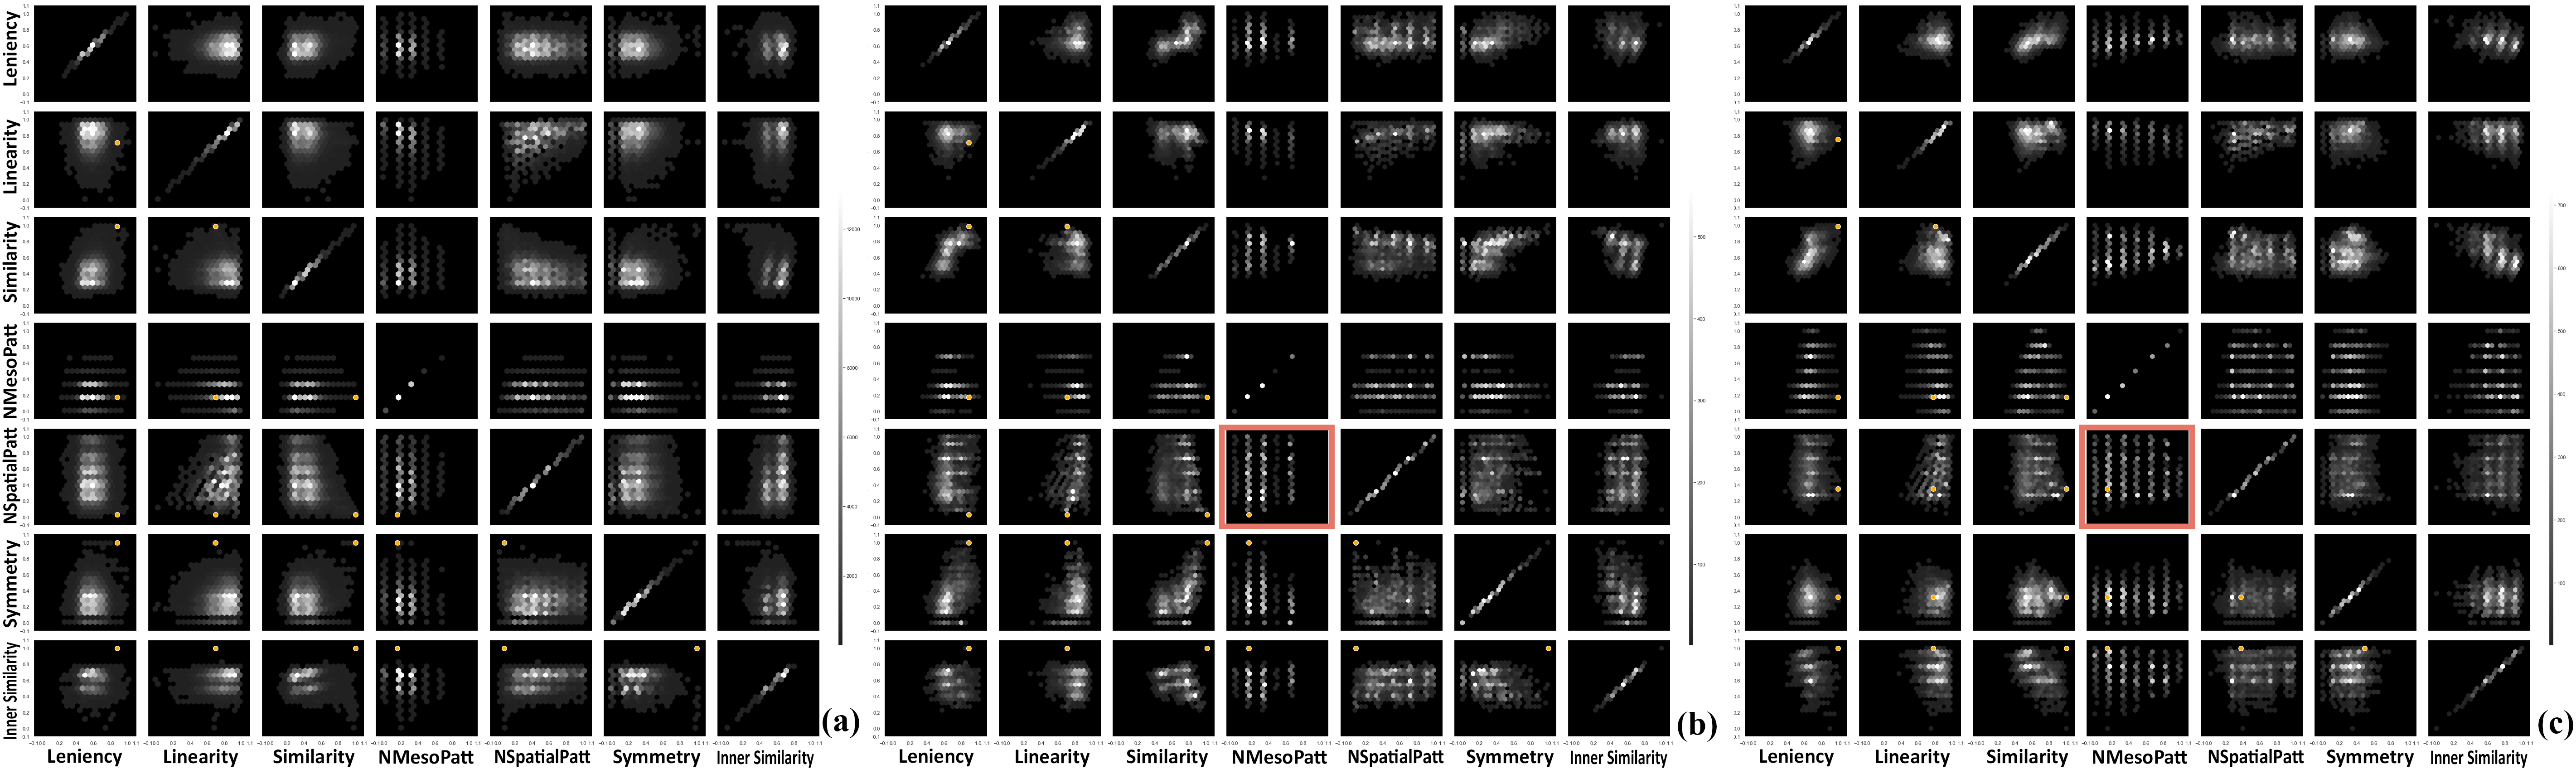
\includegraphics[width=\textwidth]{figures/figure5.png}}
\caption{In-detail run showing how all dimensions relate to each other in alternative scenarios. In (a) IC MAP-Elites ran for 2000 generations using the same target room as in \Cref{figs:full-expressive} (\Cref{figs:targetRoomsBas}), but using all the dimensions in the search, which results in 78125 cells. (b) Shows how all dimensions were explored when using~\Cref{figs:full-expressive}f (NMP-NSP) as pair of dimension. In (c) we used the same dimensions as in (b) but we changed the target room to~\Cref{figs:targetRoomsComp}. The dimensional score of the respective target room in each subfigure (\Cref{figs:targetRoomsBas} for a and b, and \Cref{figs:targetRoomsComp} for c) is highlighted with an orange mark. In b and c, the dimensions used for the experiment are highlighted with a red border.}
\label{figs:all-dimensions-earun}
\end{figure*}

\begin{figure}[h]
\centerline{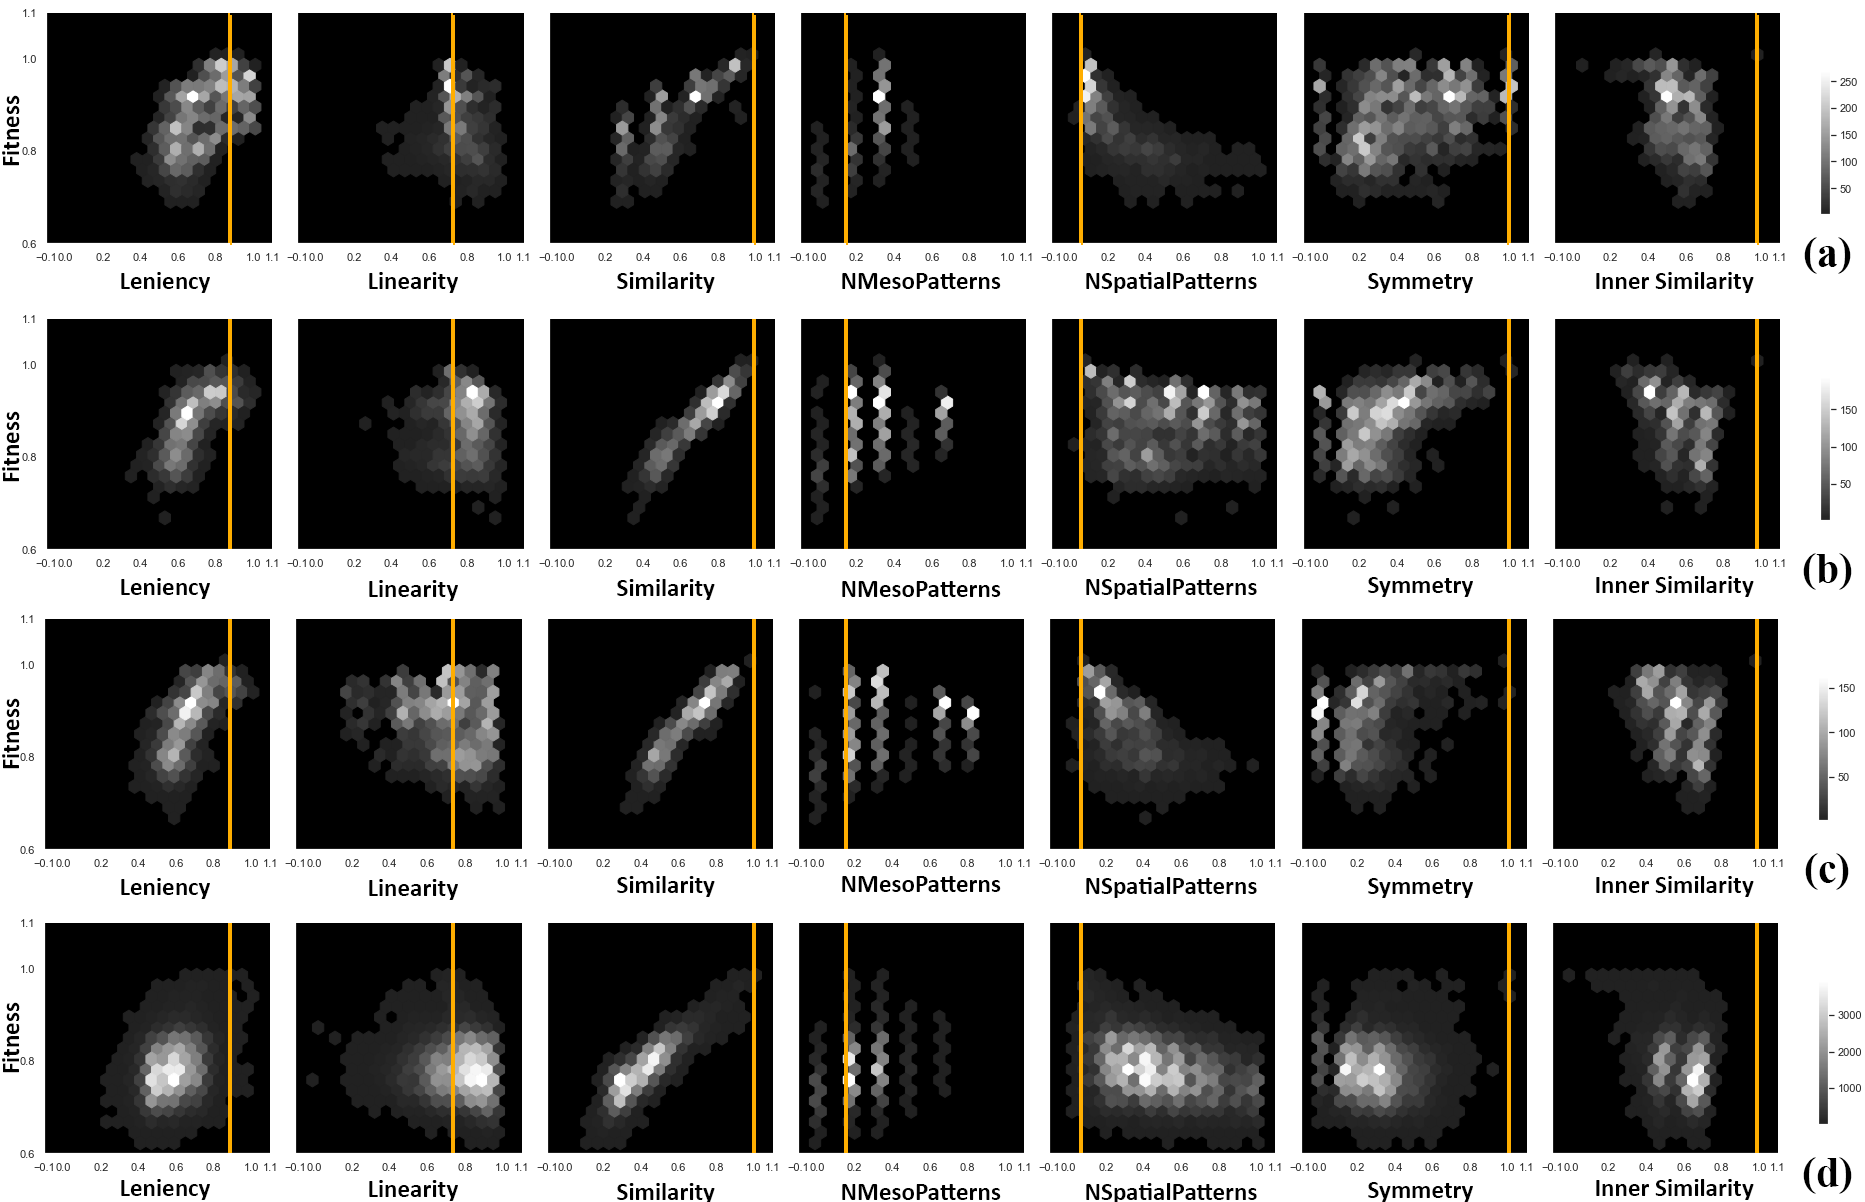
\includegraphics[width=8.5cm]{figures/figure6.png}}
\caption{Relation between dimension score and fitness score. (a), (b), and (c) show results using, respectively, Similarity and Symmetry, NMP and NSP, and NMP and Linearity. (d) was run using all the 7 dimensions. All runs used~\Cref{figs:targetRoomsBas} as target room, and it's dimensions score are denoted with an orange line across the different plots.}
\label{figs:dimensions-related-fitness}
\end{figure}

% \begin{figure}[h]
% \centerline{\includegraphics[width=7cm]{figures/fitnessTOG1.png}}
% \caption{Fitness evolution per 100 generations throughout all the runs. 
% % with continuous lines it is shown the avg. fitness, and with dashed lines it is shown the max. fitness. 
% Blue represents the fitness of the basic room (\Cref{figs:targetRoomsBas}), and Red represents the fitness of the complex room (\Cref{figs:targetRoomsComp}). 
% }
% \label{figs:avgfitness}
% \end{figure}

%One of these two options
%\begin{figure*}[h]
%\centerline{\includegraphics[width=16cm]{figures/figure-complex-room-2.png}}
%\caption{This figure shows the expressive range analysis of 3 different pair of dimensions, (a) Number of Spatial Patterns and Symmetry, (b) Number of Meso-Patterns and Symmetry, and (c) Number of Meso-Patterns and Number of Spatial Patterns. They ran using the same target room used to produce the rooms in figure \ref{figs:dimensions-example} which is a more advanced and elaborated room than the one used in figure \ref{figs:full-expressive}}
%\label{figs:expressive-range-complex}
%\end{figure*}

%\begin{figure}[t]
%\centerline{\includegraphics[width=8cm]{figures/figure-complex-room-1.png}}
%\caption{Figure is work in progress, it is missing the information of what is the value of the dimensions for the main room used to generate the data}
%\label{figs:full-expressive}
%\end{figure}
% 

%\begin{figure}[h]
%\centerline{\includegraphics[width=8cm]{figures/fig-comparison-dif-target.png}}
%\caption{This figure is work in progress since I don't know if we should use it. (a) and (b) show how different dimensions related to each other using as target dimensions Number of Meso-Patterns and Number of Spatial Patterns. The (a) side shows the EA using the simple room as target room, and the (b) side shows the EA using the more elaborated room as target room.}
%\label{figs:comparison-simple-complex}
%\end{figure}

%We have run a second set of experiments addressing...

% We ran a second set of experiments analyzing the expressive range~\cite{p6Smith:2010:Expressive-range} of the IC MAP-Elites using the 21 possible combinations of dimension pairs. We followed the same setup as presented in the previous section and every $100$ generations we collected the unique generated individuals' data, which was aggregated in all the expressive ranges and individually plotted in~\Cref{figs:avgfitness}. Through this, between $150$ to $2001$ individuals were produced every $100$ generation. By exploring the expressive range, we are able to:

% \begin{enumerate}
%     \item Analyze how and which different pairs of dimensions enable IC MAP-Elites to explore a greater range of individuals while retaining high-quality.
%     \item Conduct a comparative analysis among various dimensions.
%     \item Identify bias in the search space.
% \end{enumerate}

We ran a second set of experiments analyzing the expressive range \cite{p6Smith:2010:Expressive-range} of the IC MAP-Elites using the 21 possible combinations of dimension pairs. We followed the same setup as presented in the previous section, and every $100$ generations, we collected the unique generated individuals' data, which was aggregated in all the expressive ranges and individually plotted in~\Cref{figs:avgfitness}. Through this, between $150$ to $2001$ individuals were produced every $100$ generations. By exploring the expressive range and conducting a comparative analysis among the various dimension combinations, we intend (1) to assess IC MAP-Elites, its exploration and exploitation capabilities, and the feature dimensions, (2) to analyze how different dimension combinations affect the search for QD content, and (3) to identify bias in the search space.

Moreover, in~\Cref{tab:evaluationTable} we present a comparison of the avg. diversity and avg. quality of the generated individuals between different approaches to support our evaluation. The approaches consist of IC MAP-Elites picking dimensions in pairs (avg. of the aggregated results), IC MAP-Elites using all dimensions at the same time in the search, and the objective-based EA that was used in EDD previous to IC MAP-Elites. When using a pair of dimensions in IC MAP-Elites, the search explores in avg. $52.4$\% in the respective pair of dimensions (individual results are presented in~\Cref{figs:full-expressive}) and the individuals generated have an avg. fitness of $0.89$. In comparison, when using all dimensions rather than only pairs, the search explores $51.7$\% across all dimensions, $15$\% more than when using pairs, but with a drop in the avg. fitness of the population ($0.78$), which is discussed further in~\Cref{sec:ERAFitness} and shown in~\Cref{figs:dimensions-related-fitness}. As expected and concluded before by Mouret and Clune~\cite{p6Mouret2015}, objective-based EA generated individuals with an avg. high fitness ($0.92$), but with low diversity ($22.48$\%). This means that the search had a narrower focus, and the generated levels did not differ much from each other. Objective-based ran for $5000$ generations, but it stagnated and stopped generating novel levels after $13$ generations i.e., stopped exploring, generating a total of $1669$ levels. Conversely, IC MAP-Elites kept generating novel levels until stopped, but considerably less after $1000$ generations.

% IC MAP-Elites is by far generating more diverse levels among 

% We ran a second set of experiments analyzing the expressive range \cite{p6Smith:2010:Expressive-range} of the IC MAP-Elites using the 21 possible combinations of dimension pairs. By exploring the expressive range, we are able (1) to analyze how and which different pairs of dimensions enable IC MAP-Elites to explore a greater range of individuals while retaining high-quality, (2) to conduct a comparative analysis among various dimensions, and (3) to identify bias in the search space. We followed the same setup as presented in the previous section and every $100$ generations we collected the unique generated individuals' data, which was aggregated in all the expressive ranges and individually plotted in~\Cref{figs:avgfitness}. Through this, between $150$ to $2001$ individuals were produced every $100$ generation.%, and 4) to compare . PErhaps add some info on the fitness and dimensions

%When Smith and Whitehead~\cite{p6Smith:2010:Expressive-range} introduced the expressive range analysis of generators as an evaluation tool to examine the variety of the generated artifacts and the impact of different setups. In the paper, they highlight the importance of using comparison metrics that can measure emergent properties of the generated content. Map-Elites dimensions are features of interest in the search space that are not used to evaluate the population, rather they define the feature space of interest~\cite{p6Mouret2015}. Considering this and the previous work, we compare setups based on their behavior dimensions and on Leniency and Linearity, regardless of the used dimensions.

%Smith and Whitehead~\cite{p6Smith:2010:Expressive-range} argued that to be able to use expressive range analysis to evaluate and as a comparison tool between different setups of a generator, one must use comparison metrics that can measure emergent properties of the generated artifacts. MAP-Elites behavior dimensions are by definition emergent properties of the individuals that are not used to guide the generator (i.e. used as a fitness function) rather they are used explicitly \textbf{as an archive} to store elite individuals found in the search space. However, to be consistent with previous work, we also compared setups using Leniency and Linearity regardless of the dimensions used, besides using the behavior dimensions as comparison metrics. %, we also compared using Leniency and Linearity regardless of the dimensions used, to be consistent with previous works. %Space to cite other works that analyze the expressive range

Figure \ref{figs:full-expressive} shows the expressive range of the IC MAP-Elites with each letter referring to a unique pair of dimensions tested, and the subfigure divided into two different plots. In the left plot, we evaluate the setup based on the used pair of dimensions with each hexagon placed in relation to their dimensions' score. The hue of each of them is connected to the number of unique suggestions generated. Likewise, in the right plot, we evaluated the setup based on its linearity and leniency score, which is used to compare the setups' expressiveness. All the setups were run for $5000$ generations, using the same target room, which is shown as an orange marker (\Cref{figs:targetRoomsBas}).

In~\Cref{figs:full-expressive}, it is shown that with IC MAP-Elites, it is explored a substantial area of the generative space (denoted in the figure with $\bigcirc$ under each subfigure) rather than just exploiting the area around the target room, depicted as an orange marker. On average, in all the independent runs in their respective dimensions, the search explores around $52$\% of the space, filling at least half of the map with high-performing elites averaging $0.89$ (as shown in~\Cref{tab:evaluationTable}). It can also be observed that the dense areas of the search space (i.e., where the algorithm exploited the most) are distant from the target room's scores, and most of them are sparse throughout the search. This indicates that using IC MAP-Elites and a pair of dimensions at a time helps the distribution of the search while exploiting promising areas, and the search is less likely to be biased towards creating levels similar to the target.

Nevertheless, when using both leniency and linearity to compare the performance of the dimensions' pairs, it is shown that they are underexplored and within the same range (0.4-1.0) when not using them as dimensions. This points towards the search having difficulties getting out of other dimensions' local optima, especially since the densest search area is within the target room (this is denoted with $\bigtriangleup$ under each subfigure).


% However, using both Leniency and Linearity scores to compare the performance of the pairs of dimensions even if the dimensions were different, does not explore much of the area. 

% The dense areas of the search (i

% In average, the search explores around 49\% of the space, fill, if we average all the explored area for each independent run in their respective dimension pairs. 
% This search is around 49\% of the space, if we average all the explored area for each independent run in their respective dimension pairs. 

% We can observe that in most of the cases in \Cref{figs:full-expressive}, regardless of what pair of dimensions is used, IC MAP-Elites can explore a greater area of the search space rather than just around the target room, depicted as an orange marker in each plot, and even the dense areas of the search space (i.e. where the algorithm exploited the most) are distant from the target room's scores. Nevertheless, the expressive range shows that both leniency and linearity scores are explored within the same range (0.4-1.0) when not using any of them as dimensions, which points towards the search having difficulties getting out of other dimensions' local optima, especially since the densest search area is within the target room.

% We can observe that in most of the cases in \Cref{figs:full-expressive}, regardless of what pair of dimensions is used, IC MAP-Elites can explore a greater area of the search space rather than just around the target room, depicted as an orange marker in each plot, and even the dense areas of the search space (i.e. where the algorithm exploited the most) are distant from the target room's scores. Nevertheless, the expressive range shows that both leniency and linearity scores are explored within the same range (0.4-1.0) when not using any of them as dimensions, which points towards the search having difficulties getting out of other dimensions' local optima, especially since the densest search area is within the target room. %When using leniency or linearity as target dimensions, IC MAP-Elites finds solution in a bigger span of the

%More about the dimensions, for instance, 

\subsubsection{Alternative Scenarios}

In \Cref{figs:all-dimensions-earun}, we examine how the algorithm would vary its dimensions' exploration and exploitation in two different scenarios. (a) Using the same target room as in all the cases in \Cref{figs:full-expressive} but using all the possible dimensions in the search space (i.e. 7), and (c) using NMP and NSP (see Section~\ref{sec:dimensions}) as dimensions in the search but changing the target room to~\Cref{figs:targetRoomsComp}. To draw a better comparison, we added (b), which shows how all dimensions were explored when using~\Cref{figs:full-expressive}f (NMP-NSP) as pair of dimension.

%In \Cref{figs:all-dimensions-earun}, we examine how the algorithm would change (i.e. exploration and exploitation of the dimensions) in two different scenarios. (a) Using the same target room as in all the cases in \Cref{figs:full-expressive} but using all the possible dimensions in the search space, and (b) using NMP and NSP as dimensions in the search but changing the target room. To draw a better comparison, we added (c) which is a more detailed version of example (f) in \Cref{figs:full-expressive}, using NMP and NSP as dimensions. 

% When using all the dimensions (a), IC MAP-Elites can explore a substantial area of the search space in each of the dimensions, which is expected since all the dimensions are now acting as archives. It can also be observed that when using NMP and NSP as dimensions (b and c) regardless of the target room, the search space is greatly explored in most of the dimensions. We suspect that this is because the range between low and high scores in the NMP or NSP dimensions produces very different rooms, as it can be seen in \Cref{figs:dimensions-example} in their respective rows. 

When using all the dimensions (a), IC MAP-Elites can explore a substantial area of the search space in each of the dimensions ($51.7$\%), which in total is 15\% more searched space than when using only a pair of dimensions on average. This is expected since all the dimensions are now acting as archives. However, as it is noted in~\Cref{figs:full-expressive} under each subfigure, the actual explored space in the respective pairs ($\bigcirc$) is most of the time greater than what using all dimensions explore in the respective pair ($\dagger$).

It can also be observed that when using NMP and NSP as dimensions~\Cref{figs:all-dimensions-earun}b and c, regardless of the target room, IC MAP-Elites manages to still search a good amount of space (in avg. $38.7$\% and $43$\% among all dimensions, respectively). We suspect that this is because the range between low and high scores in the NMP or NSP dimensions produces very different rooms, as it can be seen in \Cref{figs:dimensions-example} in their respective rows. 

%When using all the dimensions (a), IC MAP-Elites can explore a big range of solutions throughout each of the dimensions used in the search, which is expected since all the dimensions are now acting as archives. It can also be observed that when using NMP and NSP as dimensions (b and c) regardless of the target room, the solution space is highly explored in most of the dimensions, which is because the range between low and high scores in the NMP or NSP dimensions yields very different rooms and combinations of micro-patterns, as it can be seen in \Cref{figs:dimensions-example} in their respective rows. 

Moreover, when comparing (a) and (b), it is noticeable that while (a) explores a greater area than (b) (in general, $15.24$\% more), %(in general, 10\% more), 
it seems to be recurrently generating the same type of individuals (i.e. depicted with the hue of the hexagon) while in (b), the dense areas for most of the dimensions are sparser, especially when matching the pair of dimensions used for evaluation. 
%This is of key importance for the fitness analysis in the following subsection, where we notice sub-optimal search-space exploitation when using all the dimensions.
 Finally, it should be noted that while these three plots are comparable in their diversity search, they differ in the number of elites they store during the search, with an archive of 78125 cells for (a), and 25 cells for (b) and (c).

% Moreover, when comparing (a) and (c), it is noticeable that while (a) can explore a more extensive area than (c), it seems to be recurrently generating the same type of individuals (i.e. depicted with the hue of the hexagon as the highly-dense areas), which in contrast in (c), the density areas for most of the dimensions are sparser, especially when matching the pair of dimensions used for evaluation. This is of key importance for the fitness analysis in the following subsection, where we notice sub-optimal search-space exploitation when using all the dimensions. Finally, it is interesting to note that these three plots, while comparable in their diversity search, differ quite drastically in the number of elites they can store during the search, with an archive of 78125 cells for (a), and 25 cells for (b) and (c). 

\subsubsection{Fitness Evaluation} \label{sec:ERAFitness}

Figure~\ref{figs:dimensions-related-fitness} shows the relation of the fitness with the explored individuals in each dimension in 4 independent runs. (a, b, c) Were runs using dimensions in pairs with the same data and dimensions as in \Cref{figs:full-expressive} (u), (f), and (h), respectively. (d) Was run using all the dimensions in the search space with the same data as in \Cref{figs:all-dimensions-earun} (a). There is an evident high correlation between Similarity scores and fitness across all the subfigures, which is expected since our fitness value is highly dependant on the target's ratios. In contrast, IS is not even close to match the fitness curve of Similarity rather there are high-performing individuals along the dimension, even when IS calculates similarity using ratios, densities, and sparsities of the target's micropatterns to calculate the score of individuals. 
% Symmetry seems to be to some extent disregarded when not used in the IC MAP-Elites search, as symmetry is overlooked in favor of exploring the other dimensions. Yet, when used  a very sensible feature dimension

% Along these lines, symmetry seems to be to some extent unstable when not used in the IC MAP-Elites search as symmetry is overlooked in favor of exploring the other dimensions. This is due to its aesthetic nature. Yet, when used in the search as in (a).

%Nevertheless, IS is not even close to match the fitness curve of Similarity, even when IS calculates similarity using ratios, densities, and sparsity of the target's micropatterns to calculate the score of individuals. This indicates that if we are not interested in aesthetically similarities, we can explore a diverse amount of high-quality individuals that retain the target's properties.

%Figure \ref{figs:dimensions-related-fitness} shows the relation of the achieved fitness with the explored individuals in each dimension in 4 independent runs. (a, b, c) Were runs using pair of dimensions, Similarity and Symmetry, NMP and NSP, and NMP and Linearity, respectively, using the same data as for \Cref{figs:full-expressive} (u), (f), and (h), respectively. (d) was run using all the dimensions in the search space using the same data as in \Cref{figs:all-dimensions-earun} (a). There is an evident high correlation between Similarity scores and fitness across all the subfigures, which is expected since our fitness value is highly dependant on the target's ratios. Nevertheless, what is more interesting is how IS does not match the fitness curve of the Similarity dimension, when IS uses ratios, densities, and sparsity of the target's micropatterns to calculate the score of individuals, in contrast with the tile by tile comparison done with Similarity. This indicates that if we disregard aesthetically similarities, we can explore a diverse amount of high-quality individuals that still contain property's similarities.

%Moreover, our experiment shows that when using specific dimensions, we achieve a relatively better search (i.e. find more diverse and high-quality individuals) on those dimensions but when not, we are still able to explore it. 

Moreover, our experiment shows that when using specific dimensions (\Cref{figs:dimensions-related-fitness}a-c), we achieve a relatively better search (i.e. find more diverse and high-quality individuals) in those dimensions, while still being able to explore the rest of dimensions. For instance, when not using NSP as a feature dimension such as in (a) or (c), the NSP dimension is fully explored but generating no high-quality individuals, meanwhile, when using NSP as a feature dimension as in (b), the search can find individuals in the same range as in (a) or (c) but with a higher fitness. 
%Similar results can be seen in the other sub figures' dimensions of interest in relation to the used behavior dimensions, as in (a) with Similarity or in (c) with Linearity.
Similar results can be seen in the rest of the dimensions where the search uses specific dimensions, for instance, in (a) exploring diverse and higher quality individuals in Similarity, or in (c) in Linearity.


%Moreover, our experiment shows that when using specific dimensions, we achieve a relatively better search (i.e. find more diverse and high-quality individuals) on those dimensions but when not, we are still able to explore it. For instance, when not using NSP as a behavior dimension such as in (a) or (c), the full spectra of dimension NSP is explored but generating no high-quality individuals, meanwhile, when using NSP as a dimension such as in (b), the search can find individuals in the same range as in (a) or (c) but with a higher fitness. A similar phenomena can be seen in the rest of the dimensions where the search uses specific dimensions (e.g. (a) exploring diverse and higher quality individuals in Similarity, and (c) in Linearity).

The most interesting result can be seen in (d), where we used all dimensions in the search. This allows for a vast search of diverse individuals in all dimensions, but at the same time it seems to exploit sub-optimal areas. On the other hand, when using only a pair of dimensions as in (a), (b) and (c), the search remained dense in high-quality individuals in all dimensions.

%Finally, the most interesting result can be seen in (d), where we used all dimensions in the search. Meanwhile, it does allow for a vast search of diverse individuals in all dimensions, it seems to exploit sub-optimal areas, which in contrast, when using only a pair of dimensions, the search remained dense in high-quality individuals in all dimensions even though the dimensions were focused on a specific pair.

\begin{figure}[h]
\centerline{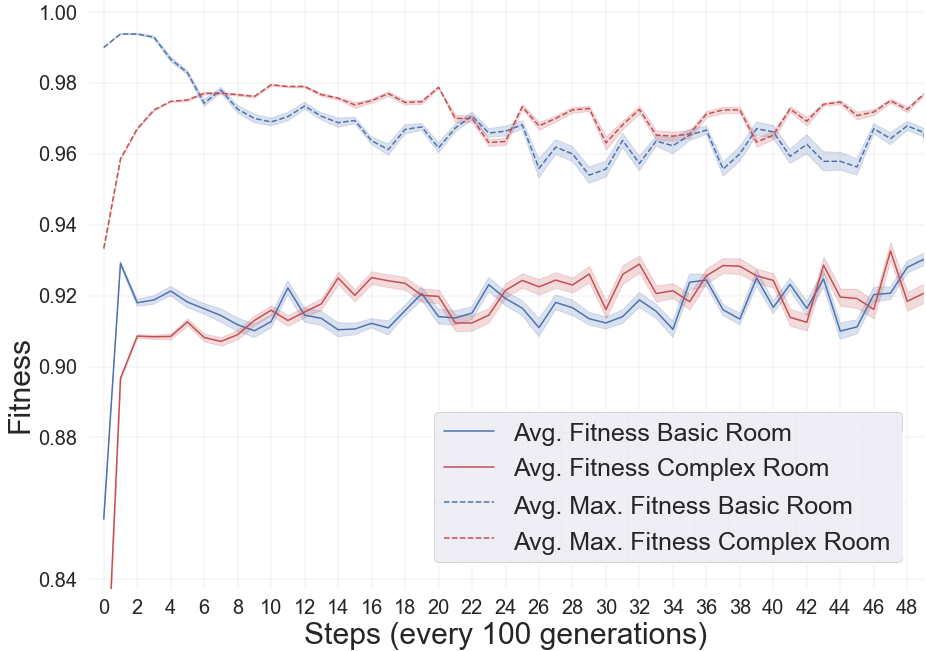
\includegraphics[width=7cm]{figures/figure7.png}}
\caption{Fitness evolution per 100 generations throughout all the runs. 
% with continuous lines it is shown the avg. fitness, and with dashed lines it is shown the max. fitness. 
Blue represents the fitness of the basic room (\Cref{figs:targetRoomsBas}), and Red represents the fitness of the complex room (\Cref{figs:targetRoomsComp}). 
}
\label{figs:avgfitness}
\end{figure}

Furthermore, figure~\ref{figs:avgfitness} shows the aggregated fitness over time of all dimension pairs (21). The avg. max fitness and the avg. total fitness are depicted as a dashed line and a continuous line, respectively. Both are surrounded by a low opacity thicker line representing the confidence interval. The graph shows that across all pairs of dimensions, the avg. fitness of novel generated levels is very high regardless of the target room and the generation, with a minor fluctuation between $0.92$ and $0.94$. In addition, the graph furthers supports what is presented in \Cref{figs:dimensions-related-fitness} a, b, and c, with most of the individuals generated in high score regions of the space in relation to fitness, but also showing that this is stable throughout the generations. The stable fitness 

This stationary overall high fitness is expected from MAP-Elites as it aims at constantly generating high-performing diverse individuals. This diversity goal, combined with an adaptive fitness dependant on the target room, makes it harder to generate levels with maximum fitness.~\Cref{figs:avgfitness} clearly shows this; depending on the fitness, there are scores in dimensions or pairs of dimensions that are less compatible with the fitness evaluation. Yet, what has been shown thus far in the multiple expressive range analysis and especially in~\Cref{figs:dimensions-related-fitness}a-c, is that IC MAP-Elites is able to generate high-performing and diverse levels. 

% However,~\Cref{figs:avgfitness} also shows that there are 

% The graph shows the avg. fitness of the novel feasible generated levels every 100 generations, which is 

% In the graph, it is plotted the newly feasible generated individuals after 100 generations

% This graph shows the fitness of the newly generated individuals after 100 generations

%Furthermore, figure~\ref{figs:avgfitness} shows the aggregated fitness over time of all dimension pairs (21). The avg. fitness is depicted as a continuous line with varying thickness, signifying the number of unique individuals generated and evaluated, and surrounding the lines with a lower opacity is the confidence interval. The graph shows that across all pairs of dimensions, the average fitness of novel generated levels is very high regardless of the target room and the generation, with a minor fluctuation between $0.92$ and $0.94$. The graph also supports what is presented in \Cref{figs:dimensions-related-fitness} a, b, and c, with most of the individuals generated in high score regions of the space in relation to fitness, but also showing that this is stable throughout the generations as expected from MAP-Elites. %Finally, as steps pass the lines become thinner

%even if the generations are very the fluctuatingin average across allall pair of dimensions the 